\documentclass[14pt]{extarticle}
\usepackage[english,ukrainian]{babel}
\usepackage[utf8]{inputenc}
\usepackage{amsmath,amssymb}
\usepackage{parskip}
\usepackage{graphicx}
\usepackage{xcolor}
\usepackage{tcolorbox}
\tcbuselibrary{skins}
\usepackage[framemethod=tikz]{mdframed}
\usepackage{chngcntr}
\usepackage{enumitem}
\usepackage{hyperref}
\usepackage{float}
\usepackage{subfig}
\usepackage{esint}
\usepackage[top=2.5cm, left=3cm, right=3cm, bottom=4.0cm]{geometry}
\usepackage[table]{xcolor}
\usepackage{algorithm}
\usepackage{algpseudocode}
\usepackage{listings}
\usepackage{xcolor}

\title{Домашня робота \#2 (перша частина) з курсу ``Комплексний аналіз''}
\author{Студента 3 курсу групи МП-31 Захарова Дмитра}
\date{\today}

\begin{document}

\maketitle

\section*{Завдання 1.}

\textbf{Умова.} Записати за допомогою нерівностей область $\mathcal{D}$, якщо її границя $\partial \mathcal{D}$ визначається кривою, що задана параметрично:
\begin{enumerate}
    \item $z = t + it^2, \; t \in (-\infty,+\infty)$;
    \item $z = \begin{cases}
        e^{i\pi t}, & t \in [0,1) \\
        t-2, & t \in [1,3]
    \end{cases}$
    \item $z=i \cos t, \; t \in [0,2\pi]$
\end{enumerate}

\subsection*{Пункт 1.}

Спочатку, зобразимо $\partial\mathcal{D}$. На комплексній площині маємо параметрично задану криву $\{\text{Re}\,z,\text{Im}\,z\}(t)=\{t,t^2\}$ для $t \in (\infty,+\infty)$. Це, очевидно, є параболою $\text{Im}\,z = (\text{Re}\, z)^2$. 

Отже, границя $\partial\mathcal{D}$ зображена на рис. \ref{fig:1_1_1}

\begin{figure}[H]
    \centering
    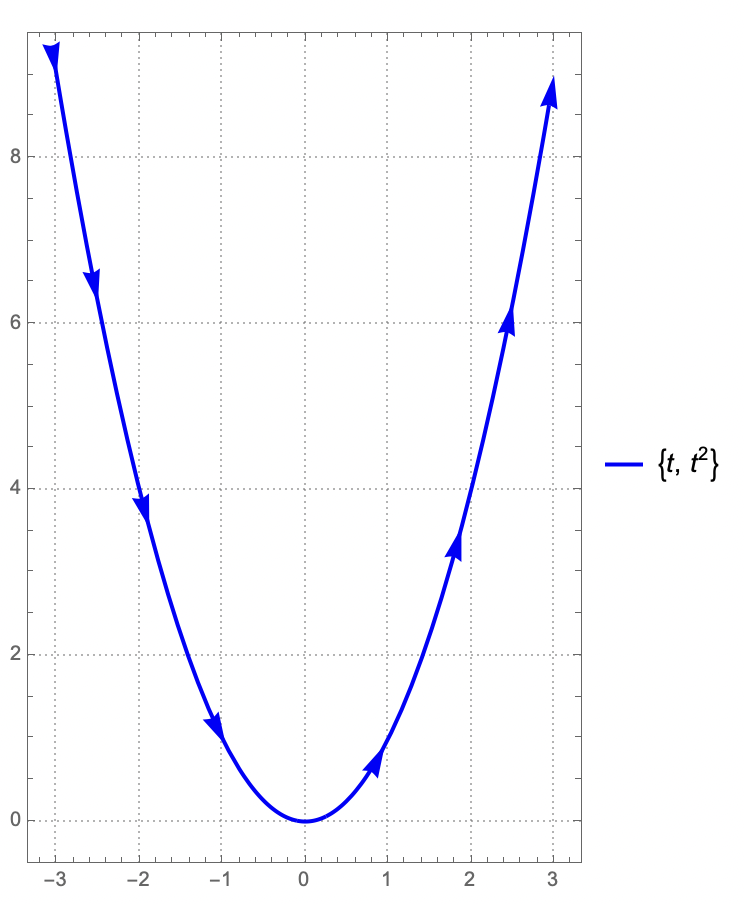
\includegraphics[width=0.5\textwidth]{images/hw_2/hw_2_1_1(1).png}
    \caption{\textcolor{blue}{Синім} відмічена границя $\partial\mathcal{D}$}
    \label{fig:1_1_1}
\end{figure}

Перевірити, що орієнтація кривої така, як на рис. \ref{fig:1_1_1}, можна наступним чином: будемо збільшувати $t$ від $0$ до $+\infty$. Тоді, на кривій $\{t,t^2\}$ абсциса та ордината буде збільшуватись, таким чином отримуємо праву гілку, починаючи з $(0,0)$. Якщо будемо навпаки, зменшувати $t$, то будемо рухатись по зменшенню абсциси, але збільшенню ординати, тобто від $(0,0)$ по лівій гілці параболи.

Сама область $\mathcal{D}$ буде знаходитись над цим графіком, оскільки в такому разі крива $\partial\mathcal{D}$ буде пробігати навколо $\mathcal{D}$ проти годинникової стрілки. Таким чином, відповідь зображена на рис. \ref{fig:1_1_2}.

Нерівність ж буде записуватись як:
\[
\text{Im} \, z > (\text{Re} \, z)^2
\]

\begin{figure}[H]
    \centering
    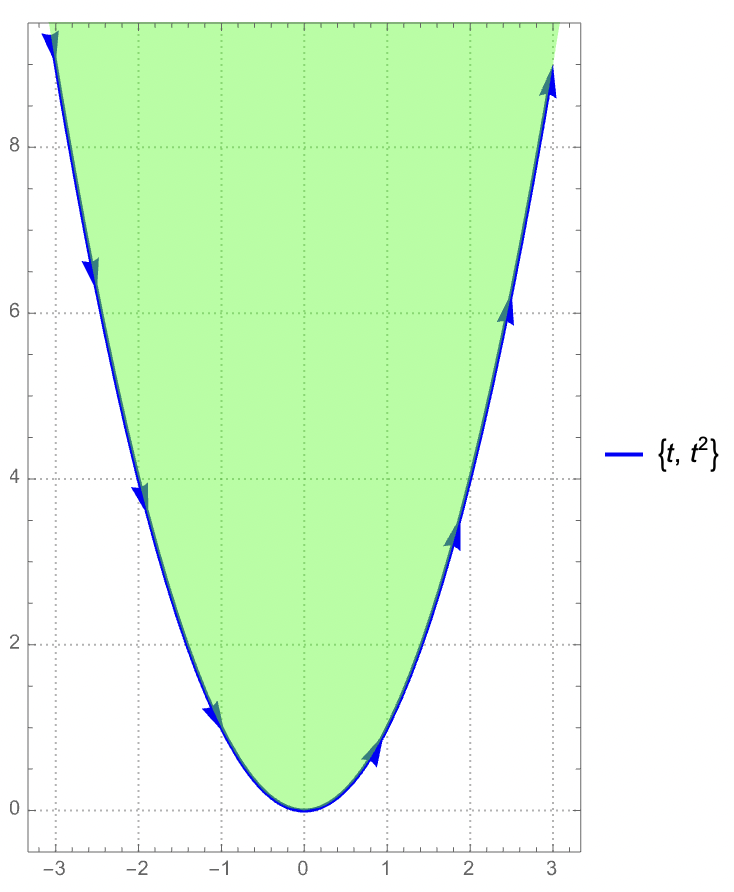
\includegraphics[width=0.5\textwidth]{images/hw_2/hw_2_1_1(2).png}
    \caption{\textcolor{blue}{Синім} відмічена границя $\partial\mathcal{D}$, \textcolor{green}{зеленим} -- область $\mathcal{D}$}
    \label{fig:1_1_2}
\end{figure}

\subsection*{Пункт 2.}

Крива $z_1(t)=e^{i\pi t}, t \in [0,1)$ є дугою одиничного кола з центром в $(0,0)$ (оскільки $z_1(t)=\cos \pi t + i\sin \pi t$, тобто в декартових координатах $\{\cos \pi t, \sin \pi t\}$). Для $t=0$ маємо $z_1(0)=1$, а для $t=1$ отримуємо $z_1(1)=\cos \pi + i \sin \pi = -1$. 

Таким чином, маємо рух по півколу $\{z\in\mathbb{C}:|z|=1 \wedge \text{Im}\, z \geq 0\}\setminus \{-1\}$ проти годинникової стрілки (без точки $-1$ оскільки $t=1$ не включено).

Крива $z_2(t)=t-2, t \in [1,3]$ є відрізком на $\text{Im}\, z = 0$ від $z_2(1)=-1$ до $z_2(3)=1$. Рух йде ``праворуч''. Ітоговий результат зображено на рис. \ref{fig:1_2_1}.

\begin{figure}[H]
    \centering
    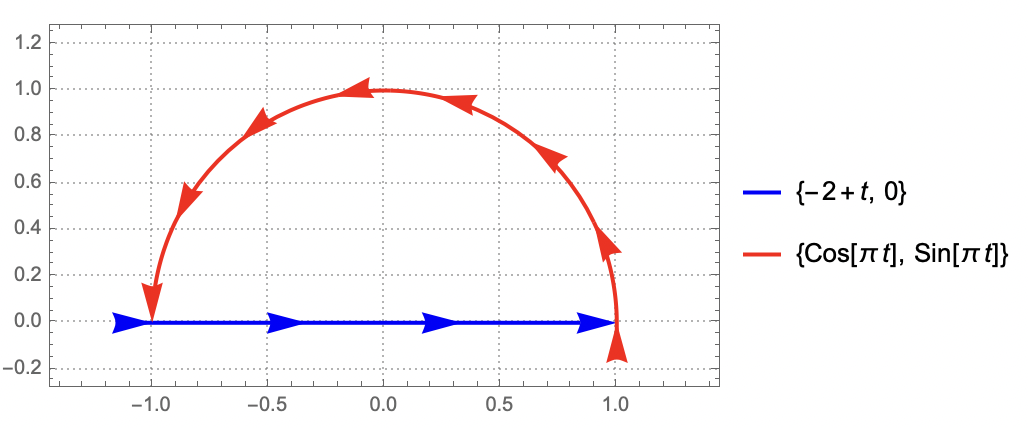
\includegraphics[width=0.9\textwidth]{images/hw_2/hw_2_1_2(1).png}
    \caption{\textcolor{red}{Червоним} відмічено криву $z_1(t)=e^{i\pi t}$, \textcolor{blue}{синім} -- криву $z_2(t)=t-2$ для відповідних границь. Для червоної кривої ми не виключали $-1$ щоб не склалось враження, що $\partial\mathcal{D}$ не містить точку $z_0=-1$.}
    \label{fig:1_2_1}
\end{figure}

Помітимо, шо $\partial\mathcal{D}$ оббігає півкруг, що міститься ``всередині'', проти годинникової стрілки. Отже, цей півкруг і є областю $\mathcal{D}$. Таким чином, відповідь зображена на рис. \ref{fig:1_2_2}, а нерівностями записується таким чином:
\[
|z| < 1 \wedge \text{Im} \, z > 0
\]

\begin{figure}[H]
    \centering
    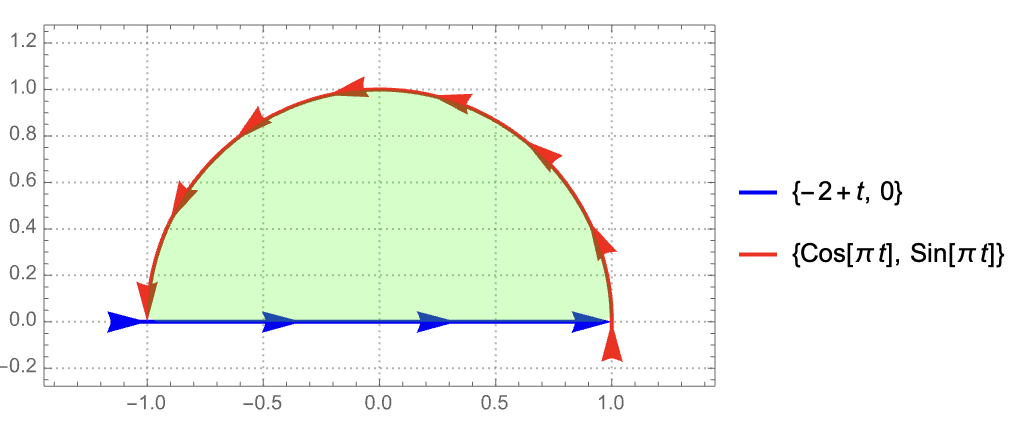
\includegraphics[width=0.9\textwidth]{images/hw_2/hw_2_1_2(2).png}
    \caption{\textcolor{red}{Червоним} відмічено криву $z_1(t)=e^{i\pi t}$, \textcolor{blue}{синім} -- криву $z_2(t)=t-2$ для відповідних границь; \textcolor{green}{зеленим} -- область $\mathcal{D}$}
    \label{fig:1_2_2}
\end{figure}

\subsection*{Пункт 3.}
$z(t)=i \cos t, \; t \in [0,2\pi]$ є відрізком на $\text{Re}\, z = 0$ (оскільки $\cos t$ -- неперервна функція). Мінімальне значення $\cos t$ на $[0,2\pi]$ це $-1$, а максимальне $1$, тому це відрізок від $-i$ до $+i$. Цю множину можна записати як:
\[
\partial\mathcal{D} = \{z \in \mathbb{C}: \text{Re}\, z = 0 \wedge |\text{Im}\, z| \leq 1\}
\]

Область $\mathcal{D} = \overline{\partial\mathcal{D}}$. Запишемо:
\begin{align*}
\mathcal{D} = \{z \in \mathbb{C}: \overline{\text{Re}\, z = 0 \wedge |\text{Im}\, z| \leq 1}\}  \\
=\{z \in \mathbb{C}: \text{Re} \, z \neq 0 \vee |\text{Im} \, z| > 1\}
\end{align*}

Таким чином маємо нерівність $\text{Re}\, z \neq 0 \vee |\text{Im}\, z| > 1$. 

\textbf{Відповідь.}

\textbf{Пункт 1.} $\text{Im}\, z > (\text{Re}\,z)^2$.

\textbf{Пункт 2.} $|z|<1 \wedge \text{Im}\, z > 0$.

\textbf{Пункт 3.} $\text{Re}\, z \neq 0 \vee |\text{Im}\, z| > 1$.

\section*{Завдання 2.} 

\textbf{Умова.} Нехай $\text{Re}\, f=u$. Відновити аналітичну функцію $f(x+iy)=u(x,y)+iv(x,y)$:
\begin{enumerate}
    \item $u(x,y)=x^2-y^2+xy$;
    \item $u(x,y)=x^3+6x^2y-3xy^2-2y^3, \; f(0)=0$.
\end{enumerate}

\textbf{Розв'язок.} За означенням, функція є аналітичною тоді, коли вона є $\mathbb{C}$-диференційованою. Отже, мають виконуватися умови Коші-Рімана. Інакшими словами:
\[
u_x' = v_y' \wedge u_y' = -v_x'
\]

Далі потрібно розв'язати цю систему диференціальних рівнянь відносно $v(x,y)$. Для цього спочатку інтегруємо перше рівняння:
\[
v_y' = u_x' \implies v = \int u_x'(x,y)dy
\]

і підставляємо результат у друге.

\subsection*{Пункт 1.} 

Розписавши, маємо:
\[
\begin{cases}
    v_y' = 2x+y \\
    v_x' = 2y-x
\end{cases}
\]

З першого рівняння $v(x,y) = 2xy + \frac{y^2}{2} + \varphi(x)$. Підставляючи у друге, маємо:
\[
2y + \varphi'(x) = 2y - x \implies \varphi'(x) = -x \implies \varphi(x) = -\frac{x^2}{2}+C
\]

Отже, остаточно отримуємо
\[
v(x,y) = -\frac{x^2}{2} + \frac{y^2}{2} + 2xy + C
\]

\subsection*{Пункт 2.} 

Знову підставляємо умову Коші-Рімана:
\[
\begin{cases}
    v_y' = 3x^2+12xy-3y^2 \\
    v_x' = 6y^2+6xy-6x^2 
\end{cases}
\]

Інтегруємо:
\[
v = 3x^2y + 6xy^2 - y^3 + \varphi(x)
\]

Підставляємо у друге:
\[
6xy + 6y^2 + \varphi'(x) = 6y^2 + 6xy - 6x^2 \implies \varphi'(x) = -6x^2 \implies \varphi(x) = -2x^3 + C
\]

Отже:
\[
v(x,y) = 3x^2y + 6xy^2 - y^3 - 2x^3 + C
\]

Також використаємо умову, що $f(0)=0$. Ця умова еквівалентна $u(0,0)=v(0,0)=0$. Одразу видно, що $u(0,0)=0$, а $v(0,0)=C$. Отже, $C=0$. Тому остаточно
\[
v(x,y) = -2x^3-y^3+3x^2y+6xy^2
\]

\textbf{Відповідь.} 

1. $v(x,y)=-\frac{x^2}{2}+\frac{y^2}{2}+2xy+C$. 
2. $v(x,y)=-2x^3-y^3+3x^2y+6xy^2$

\end{document}

